%%
%% This is file `docultex.tex', 
%% Documentation for siam supplemental file macros for use with LaTeX 2e
%% 
%% December 19, 2013
%%
%% Supplemental Files Supported Version 1.0.0
%% 
%% You are not allowed to change this file. 
%% 
%% You are allowed to distribute this file under the condition that 
%% it is distributed together with all of the files in the siam macro 
%% distribution. These are:
%%
%%  siamltex1213.cls (main LaTeX macro for SIAM)
%%  siam10.clo   (size option for 10pt papers)
%%  subeqn.clo   (allows equation numbners with lettered subelements)
%%  siam.bst     (bibliographic style file for BibTeX)
%%  docultex.tex (this file)
%%
%% If you receive only some of these files from someone, complain! 
%% 
%% You are NOT ALLOWED to distribute this file alone. You are NOT 
%% ALLOWED to take money for the distribution or use of either this 
%% file or a changed version, except for a nominal charge for copying 
%% etc. 
%% \CharacterTable
%%  {Upper-case    \A\B\C\D\E\F\G\H\I\J\K\L\M\N\O\P\Q\R\S\T\U\V\W\X\Y\Z
%%   Lower-case    \a\b\c\d\e\f\g\h\i\j\k\l\m\n\o\p\q\r\s\t\u\v\w\x\y\z
%%   Digits        \0\1\2\3\4\5\6\7\8\9
%%   Exclamation   \!     Double quote  \"     Hash (number) \#
%%   Dollar        \$     Percent       \%     Ampersand     \&
%%   Acute accent  \'     Left paren    \(     Right paren   \)
%%   Asterisk      \*     Plus          \+     Comma         \,
%%   Minus         \-     Point         \.     Solidus       \/
%%   Colon         \:     Semicolon     \;     Less than     \<
%%   Equals        \=     Greater than  \>     Question mark \?
%%   Commercial at \@     Left bracket  \[     Backslash     \\
%%   Right bracket \]     Circumflex    \^     Underscore    \_
%%   Grave accent  \`     Left brace    \{     Vertical bar  \|
%%   Right brace   \}     Tilde         \~}

\documentclass[final,leqno,onefignum,onetabnum]{siamltex1213}

\usepackage{graphicx}
%% \graphicspath{ {"/Users/hogstrom/Dropbox (Personal)/cources_spring_2015_MIT/18_335_Numeric_Methods/NMF/figures/"} }
\graphicspath{ {/Users/hogstrom/Documents/code/ThornsInRoses/18_335} }
\DeclareGraphicsExtensions{.pdf,.png,.jpg}

\title{USING SIAM'S \LaTeX\ MACROS\thanks{This work was
supported by the Society for Industrial and Applied
Mathematics}} 

\author{TeX Production\thanks{Society for Industrial and
Applied Mathematics, Philadelphia, Pennsylvania. 
(\email{tex@siam.org}). Questions, comments, or corrections
to this document may be directed to that email address.}}

\begin{document}
\maketitle
\slugger{mms}{xxxx}{xx}{x}{x--x}%slugger should be set to mms, siap, sicomp, sicon, sidma, sima, simax, sinum, siopt, sisc, or sirev

\begin{abstract}
Documentation is given for use of the SIAM \LaTeX\ macros. These
macros are now compatible with \LaTeX$2_{\varepsilon}$.
Instructions and suggestions for compliance with SIAM style
standards are also included. Familiarity with standard \LaTeX\ commands
is assumed.
\end{abstract}

\begin{keywords}\end{keywords}

\begin{AMS}\end{AMS}


\pagestyle{myheadings}
\thispagestyle{plain}
\markboth{TEX PRODUCTION}{USING SIAM'S \LaTeX\ MACROS}

\section{Introduction}

This file is documentation for the SIAM \LaTeX\ macros, and
provides instruction for submission of your files.

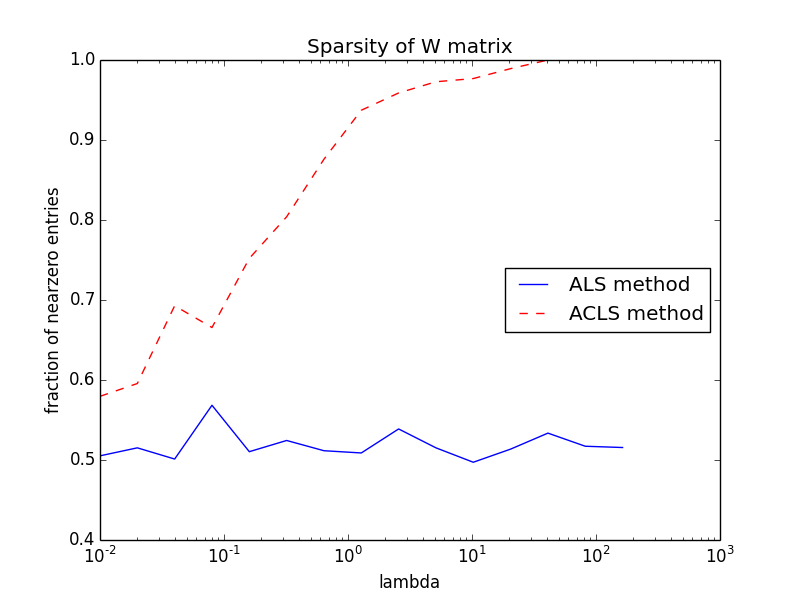
\includegraphics[width=0.4\textwidth,natwidth=800,natheight=600]{ALS_vs_ACLS_sparsity.png}


To accommodate authors who electronically typeset their manuscripts,
SIAM supports the use of \LaTeX. To ensure quality typesetting according
to SIAM style standards, SIAM provides a \LaTeX\ macro style file.
Using \LaTeX\ to format a manuscript should simplify the editorial process
and lessen the author's proofreading burden. However,
it is still necessary to proofread the galley proofs with care.

Electronic files should not be submitted until the paper has been
accepted, and then not until requested to do so by someone in the SIAM
office. Once an article is slated for an issue,
someone from the SIAM office will contact the author about any or all
of the following: editorial and stylistic queries, 
supplying the source files (and any supplementary macros)
for the properly formatted article, and handling figures.

When submitting electronic files  (electronic submissions) 
(to {\tt tex@siam.org}) include  the journal, issue, and author's
name in the subject line of the message. 
Authors are responsible for ensuring  that the paper generated 
from the source files exactly matches the paper that
was accepted for publication by the review editor. If it does not,
information on how it differs should be indicated in the transmission 
of the file. When submitting a file, please be sure to include any 
additional macros (other than those provided by SIAM) that will be 
needed to run the paper. 

SIAM uses MS-DOS-based computers for \LaTeX\ processing. Therefore
all filenames should be restricted to eight characters or less,
plus a three character extension.

Once the files are corrected here at SIAM, we will mail the revised 
proofs to be read against the original edited hardcopy 
manuscript. We are not
set up to shuttle back and forth varying electronic versions of each
paper, so we must rely on hard copy of the galleys. The author's proofreading
is an important but easily overlooked step. Even if SIAM were not
to introduce a single editorial change into your manuscript, there
would still be a need to check, because electronic transmission
can introduce errors.

The distribution contains the following items: {\tt
siamltex1213.cls}, the main macro package based on {\tt
article.cls}; {\tt siam10.clo}, for the ten-point size option;\linebreak 
{\tt subeqn.clo}, a style option for equation numbering (see \S3 for
an explanation); and  {\tt siam.bst},
 the style file for use with {\sc Bib}\TeX. Also included, of course, is this
file {\tt docultex.tex}.
The rest of this paper will highlight
some keys to effective macro use, as well as point out options and
special cases, and describe SIAM style standards to which
authors should conform.


\section{Headings}
The top matter of a journal paper falls into a standard
format. It begins of course with the \verb|\documentclass| command

\begin{verbatim}

\documentclass{siamltex1213}

\end{verbatim}

Other class options  can be included
in the bracketed argument of the command, separated by commas.

Suggested optional arguments include:
\begin{description}
\item[final] Without this option, lines which extend past the
margin will have black boxes next to them to help authors identify
lines that they need to fix, by re-writing or inserting breaks. \verb|final|
turns these boxes off, so that very small margin breaks which are not
noticible will not cause boxes to be generated.

\item[oneeqnum] Normally \verb|siamltex.cls| numbers equations,
tables, figures, and theorem environments with a decimal number, 
composed of the section of the paper, a period, and the number of
the enumerated object (example: 1.2). The sequence of numbering
is also restarted with each new section, so that, for example, the last
equation of section 3 may be 3.10, but the first equation of section
4 would be 4.1. Using \verb|oneeqnum| numbers all equations consecutively
throughout a paper with a single digit.

\item[onethmnum] Using \verb|onethmnum| numbers all theorem-like
environments consecutively throughout a paper with a single digit.

\item[onefignum] Using \verb|onethmnum| numbers all figures
 consecutively throughout a paper with a single digit.

\item[onetabnum] Using \verb|onethmnum| numbers all tables
 consecutively throughout a paper with a single digit.
\end{description}

The title and author parts are formatted using the
\verb|\title| and \verb|\author| commands as described in Lamport
\cite{Lamport}. The \verb|\date|
command is not used. \verb|\maketitle| produces the actual
output of the commands.

The addresses and support acknowledgments are put into the
\verb|\author| commands via \verb|\thanks|. If support is
overall for the authors, the support acknowledgment should
be put in a \verb|\thanks| command in the \verb|\title|.
Specific support should go following the addresses of the
individual authors in the same \verb|\thanks| command.

Sometimes authors have support or addresses in common which
necessitates having multiple \verb|\thanks| commands for
each author. Unfortunately \LaTeX\ does not normally allow this, 
so a special procedure must be used. An example of this procedure
follows. Grant information can also be run into both authors' 
footnotes.

\begin{verbatim}

\title{TITLE OF PAPER}

\author{A.~U. Thorone\footnotemark[2]\ \footnotemark[5]
\and A.~U. Thortwo\footnotemark[3]\ \footnotemark[5]
\and A.~U. Thorthree\footnotemark[4]}

\begin{document}
\maketitle

\renewcommand{\thefootnote}{\fnsymbol{footnote}}

\footnotetext[2]{Address of A.~U. Thorone}
\footnotetext[3]{Address of A.~U. Thortwo}
\footnotetext[4]{Address of A.~U. Thorthree}
\footnotetext[5]{Support in common for the first and second
authors.}

\renewcommand{\thefootnote}{\arabic{footnote}}

\end{verbatim}

Notice that the footnote marks begin with {\tt [2]}
because the first mark (the asterisk) will be used in the
title for date-received information by SIAM, even if not
already used for support data. This is just one example;
other situations follow a similar pattern.

Following the author and title is the abstract, key words
listing, and AMS subject classification number(s),
designated using the \verb|{abstract}|, \verb|{keywords}|,
and \verb|{AMS}| environments. If
there is only one AMS number, the commands
\verb|\begin{AM}| and \verb|\end{AM}| are used
instead of \verb|{AMS}|. This causes the heading to be
in the singular. Authors are responsible for providing AMS numbers.
They can be found in the Annual Index of Math Reviews, or
through {\tt e-Math} ({\tt telnet e-math.ams.com}; login
and password are both {\tt e-math}).   

Left and right running heads should be provided in the
following way.

\begin{verbatim}

\pagestyle{myheadings}
\thispagestyle{plain}
\markboth{A.~U. THORONE AND A.~U. THORTWO}{SHORTER PAPER TITLE} 

\end{verbatim}

\section{Equations and mathematics}

One advantage of \LaTeX\ is that it can automatically number
equations and refer to these equation numbers in text. While plain \TeX's
method of equation numbering (explicit numbering using
\verb|\leqno|) works in the SIAM macro, it is not preferred
except in certain cases. SIAM style guidelines call for
aligned equations in many circumstances, and \LaTeX's 
\verb|{eqnarray}| environment is not compatible with
\verb|\leqno| and \LaTeX\ is not compatible with the plain
\TeX\ command \verb|\eqalign| and \verb|\leqalignno|. Since
SIAM may have to alter or realign certain groups of
equations, it is necessary to use the \LaTeX\ system of
automatic numbering.

Sometimes it is desirable to designate subequations of a larger
equation number. The subequations are designated with
(roman font) letters appended after the number. SIAM has
supplemented its macros with the {\tt subeqn.clo} option which
defines the environment \verb|{subequations}|.

\begin{verbatim}

\begin{subequations}\label{EKx}
\begin{equation}
 y_k =  B  y_{k-1} +  f, \qquad k=1,2,3,\ldots  
\end{equation}
for  any initial vector $ y_0$.   Then 
\begin{equation}
 y_k\rightarrow  u \mbox{\quad iff\quad} \rho( B)<1.
\end{equation}
\end{subequations}

\end{verbatim}

All equations within the \verb|{subequations}| environment
will keep the same overall number, but the letter
designation will increase.

Clear equation formatting using \TeX\ can be challenging. Aside from
the regular \TeX\ documentation, authors will find Nicholas 
J. Higham's book {\em Handbook of Writing for the Mathematical
Sciences\/} \cite{Higham} useful for guidelines and tips on 
formatting with \TeX. The book covers many other topics related 
to article writing as well.                

Authors commonly make mistakes by using
 \verb|<|, \verb|>|, \verb|\mid|, and 
\verb|\parallel| as delimiters, instead of 
\verb|\langle|, \verb|\rangle|, \verb:|:,
and \verb:\|:. The incorrect symbols have particular 
meanings distinct from the correct ones and should not be confused.

\begin{table}[htbp]
\caption{Illustration of incorrect delimiter use.}
\begin{center}\footnotesize
\renewcommand{\arraystretch}{1.3}
\begin{tabular}{|ll|ll|}\hline
\multicolumn{2}{|c|}{{\bf Wrong}} & \multicolumn{2}{c|}{{\bf Right}}\\ \hline
\verb|<x, y>| & $<x, y>$   &  \verb|\langle x, y\rangle| & $\langle x, y\rangle$\\
\verb|5 < \mid A \mid| &  $5 < \mid A \mid$ & \verb:5 < |A|: &  $5 < |A|$\\
\verb|6x = \parallel x|&&&\\ 
\verb|    - 1\parallel_{i}| & $6x = \parallel x - 1\parallel_{i}$ &
   \verb:6x = \|x - 1\|_{i}: & $6x = \| x - 1\|_{i}$\\ \hline
\end{tabular}
\end{center}
\end{table}

Another common author error is to put large (and even medium sized)
matrices in-line with the text, rather than displaying them. This
creates unattractive line spacing problems, and should be assiduously
avoided. Text-sized matrices (like $({a \atop b} {b \atop c})$) might
be used but anything much more complex than the example cited will
not be easy to read and should be displayed.

More information on the formatting of equations and aligned
equations is found in Lamport \cite{Lamport}. Authors bear 
primary responsibility for formatting their equations within 
margins and in an aesthetically pleasing and informative manner.

The SIAM macros include additional roman math words, or ``log-like"
functions, to those provided in standard \TeX.  The following
commands are added: \verb:\const:, \verb:\diag:, \verb:\grad:,
\verb:\Range:, \verb:\rank:, and \verb:\supp:.
These commands produce the same word as the command name
in math mode, in upright type.

\section{Special fonts}

SIAM supports the use of the AMS-\TeX\ fonts (version 2.0
and later). The package \verb|amsfonts| can be included with
the command\linebreak \verb|\usepackage{amsfonts}|. This package
is part of the AMS-\LaTeX distribution, available
from the AMS or from the Comprehensive TeX Archive
Network (anonymous ftp to ftp.shsu.edu). The blackboard bold font in this
font package can be used for designating number sets. 
This is preferable to other methods of combining letters
(such as I and R for the real numbers) to produce pseudo-bold
letters but this is tolerable as well. Typographically speaking,
number sets may simply be designated using regular bold letters; 
the blackboard bold typeface was designed to fulfil a desire
to simulate the limitations of a chalk board in printed type.


\subsection{Punctuation}
All standard punctuation and all numerals should be set in roman type
(upright) even within italic text. The only exceptions are periods and 
commas. They may be set to match the surrounding text.

References to sections should use the symbol \S, generated by
\verb|\S|. (If the reference begins a sentence, the term ``Section''
should be spelled out in full.) Authors should not redefine
\verb|\S|, say, to be a calligraphic S, because \verb|\S|
must be reserved for use as the section symbol.  

Authors sometimes confuse the use of various types of dashes.
Hyphens (\verb|-|, -) are used for some compound words (many
such words should have no hyphen but must be run together, 
like ``nonzero,'' or split apart, like ``well defined''). 
Minus signs (\verb|$-$|, $-$)
should be used in math to represent subtraction or negative numbers.
En dashes (\verb|--|, --) are used for ranges (like 3--5, 
June--August), or for joined names (like Runge--Kutta). Em dashes
(\verb|---|, ---) are used to set off a clause---such as this 
one---from the rest of the sentence. 


\subsection{Text formatting}

SIAM style preferences do not make regular use of the \verb|{enumerate}|
and \verb|{itemize}| environments. Instead,
{\tt siamltex.cls} includes definitions of two alternate list
environments, \verb|{remunerate}| and \verb|{romannum}|.
Unlike the standard itemized lists, these environments do
not indent the secondary lines of text. The labels, whether
defaults or the optional user-defined, are always aligned
flush right.

The \verb|{remunerate}| environment consecutively numbers
each item with an arabic numeral followed by a period. This
number is always upright, even in slanted
environments. (For those wondering at the unusual
naming of this environment, it comes from Seroul and Levy's
\cite{SerLev} definition of a similar macro for plain \TeX: 
%{\tt \char"5C meti} 
\verb|\meti| which is
% {\tt \char"5C item}
\protect\verb|\item|  spelled backwards. Thus
%{\tt \{remunerate\}}, 
\verb|{remunerate}|
a portion of 
%{\tt \{enumerate\}}
\verb|{enumerate}|
spelled backwards.)

The \verb|{romannum}| environment consecutively numbers
each item with a lower-case roman numeral enclosed in
parentheses. This number will always be upright within
slanted environments (as in theorems).


\section{Theorems and Lemmas}
Theorems, lemmas, corollaries, definitions, and propositions are covered
in the SIAM macros by the theorem-environments
\verb|{theorem}|, \verb|{lemma}|, \verb|{corollary}|,
\verb|{definition}| and \verb|{proposition}|. These are all
numbered in the same sequence and produce labels in small 
caps with an italic body. Other environments may be specified by the
\verb|\newtheorem| command. SIAM's style is for Remarks and Examples
to appear with italic labels and an upright roman body.

\begin{verbatim}

\begin{theorem}
Sample theorem included for illustration.  
Numbers and parentheses, like equation $(3.2)$, should be set 
in roman type.  Note that words (as opposed to ``log-like''
functions) in displayed equations, such as
$$ x^2 = Y^2 \sin z^2 \mbox{ for all } x $$
will appear in italic type in a theorem, though normally
they should appear in roman.\end{theorem}

\end{verbatim}

This sample produces Theorem 4.1 below.

\begin{theorem}
Sample theorem included for illustration.  
Numbers and parentheses, like equation $(3.2)$, should be set 
in roman type.  Note that words (as opposed to ``log-like''
functions) in displayed equations, such as
$$ x^2 = Y^2 \sin z^2 \mbox{ for all } x $$
will appear in italic type in a theorem, though normally
they should appear in roman.
\end{theorem}


Proofs are handled with the \verb|\begin{proof}|
\verb|\end{proof}| environment. A ``QED'' box \endproof\ is created
automatically by \verb|\end{proof}|, but this should be
preceded with a \verb|\qquad|.

Named proofs, if used, must be done independently by the
authors. SIAM style specifies that proofs which end with
displayed equations should have the QED box two ems (\verb|\qquad|)
from the end of the equation on line with it horizontally.
Below is an example of how this can be done:

\begin{verbatim}

{\em Proof}. Proof of the previous theorem 
                .
                .
                .
thus,
$$
a^2 + b^2 = c^2 \qquad\endproof
$$

\end{verbatim}


\section{Figures and tables}
Figures and tables sometimes require special consideration.
Tables in SIAM style are need to be set in eight point size
by using the \verb|\footnotesize| command inside the 
\verb|\begin{table}| environment. Also, they should be designed 
so that they do not extend beyond the text margins. 

SIAM style requires that no figures or tables  appear in the
references section of the paper. \LaTeX\ is notorious for
making figure placement difficult, so it is important to
pay particular attention to figure placement near the
references in the text. All figures and tables should
be referred to in the text.

SIAM supports the use of {\tt epsfig} for including {\sc PostScript}
figures. All {\sc Post\-Script} figures should be sent in separate
files. See the {\tt epsfig} documentation (available via
anonymous ftp from CTAN: ftp.shsu.edu) for more details on the use
of this style option. It is a good idea to submit high-quality
hardcopy of all {\sc Post\-Script} figures just in case there 
is difficulty in the reproduction of the figure. Figures produced 
by other non-\TeX\ methods should be included as high-quality 
hardcopy when  the manuscript is submitted.

{\sc PostScript} figures that are sent should be generated with
sufficient line thickness. Some past figures authors have sent
had their line widths become very faint when SIAM set the papers
using a high-quality 1200dpi printer.

Hardcopy for non-{\sc PostScript} figures should be included in
the submission of the hardcopy of the manuscript. Space
should be left in the \verb|{figure}| command for the
hardcopy to be inserted in production.

\section{Bibliography and Bib\TeX}

If using {\sc Bib}\TeX, authors need not submit the {\tt .bib} file for
their papers. Merely submit the completed {\tt .bbl} file, having used
{\tt siam.bst} as their bibliographic style file. {\tt siam.bst}
only works with Bib\TeX\ version 99i and later. The use of
Bib\TeX\ and the preparation of a {\tt .bib} file is
described in greater detail in \cite{Lamport}.

If not using Bib\TeX, SIAM bibliographic references follow
the format of the following examples:

\begin{verbatim}

\bibitem{Ri} {\sc W. Riter},
{\em Title of a paper appearing in a book}, in The Book 
Title, E.~D. One, E.~D. Two, and A.~N. Othereditor, eds., 
Publisher, Location, 1992, pp.~000--000.

\bibitem{AuTh1} {\sc A.~U. Thorone}, {\em Title of paper
with lower case letters}, SIAM J. Abbrev. Correctly, 2
(1992), pp.~000--000.

\bibitem{A1A2} {\sc A.~U. Thorone and A.~U. Thortwo}, {\em
Title of paper appearing in book}, in Book Title: With All
Initial Caps, Publisher, Location, 1992.

\bibitem{A1A22} \sameauthor, % generates the 3 em rule
{\em Title of Book{\rm :} Note Initial Caps and {\rm ROMAN
TYPE} for Punctuation and Acronyms}, Publisher,
Location, pp.~000--000, 1992.

\bibitem{AuTh3} {\sc A.~U. Thorthree}, {\em Title of paper
that's not published yet}, SIAM. J. Abbrev. Correctly, to appear.

\end{verbatim}

Other types of references fall into the same general
pattern. See the sample file or any SIAM journal for other
examples. Authors must correctly format their bibliography to
be considered as having used the macros correctly. An incorrectly 
formatted bibliography is not only time-consuming for SIAM to
process but it is possible that errors may be introduced into 
it by keyboarders/copy editors.

As an alternative to the above style of reference, an alphanumeric
code may be used in place of the number (e.g., [AUTh90]). The same
commands are used, but \verb|\bibitem| takes an optional argument
containing the desired alphanumeric code. 

Another alternative is no number, simply the authors' names and
the year of publication following in parentheses. The rest of the
format is identical. The macros do not support this alternative
directly, but modifications to the macro definition are possible
if this reference style is preferred.


\section{Conclusion} Many other style suggestions and tips
could be given to help authors but are beyond the scope of this
document. Simple mistakes can be avoided by increasing your familiarity
with how \LaTeX\ functions. The books referred to throughout this document
are also useful to the author who wants clear, beautiful typography
with minimal mistakes. 

\Appendix
\section{The use of appendices}
The \verb|\appendix| command may be used before the final sections
of a paper to designate them as appendices. Once \verb|\appendix|
is called, all subsequent sections will appear as 

\appendix
\section{Title of appendix} Each one will be sequentially lettered
instead of numbered. Theorem-like environments, subsections,
and equations will also have the section number changed to a letter.

If there is only {\em one} appendix, however, the \verb|\Appendix|
(with a capital letter) should be used instead. This produces only 
the word {\bf Appendix} in the section title, and does not add a letter.
Equation numbers, theorem numbers and subsections of the appendix
will have the letter ``A''  designating the section number.

If you don't want to title your appendix, and just call it
{\bf Appendix A.} for example, use \verb|\appendix\section*{}| 
and don't include anything in the title field. This works
opposite to the way \verb|\section*| usually works, by including the
section number, but not using a title.

 
Appendices should appear before the bibliography section, not after,
and any acknowledgments should be placed after the appendices and before
the bibliography. 

\begin{thebibliography}{1}
\bibitem{GoMiSa} {\sc M. Goossens, F. Mittelbach, and A. Samarin},
{\em The} \LaTeX\ {\em Companion}, Addison-Wesley, Reading, MA, 1994.

\bibitem{Higham} {\sc N.~J. Higham}, {\em Handbook of Writing for
the Mathematical Sciences}, Society for Industrial and Applied
Mathematics, Philadelphia, PA, 1993.

\bibitem{Lamport} {\sc L. Lamport}, \LaTeX: {\em A Document
Preparation System}, Addison-Wesley, Reading, MA, 1986.

\bibitem{SerLev} {\sc R. Seroul and S. Levy}, {\em A
Beginner's Book of} \TeX, Springer-Verlag, Berlin, New
York, 1991.
\end{thebibliography}


\end{document}
%% end of file `docultex.tex'
